\documentclass[tikz]{standalone} % สั่งให้เป็นไฟล์แยกที่ compile ได้เอง
\usepackage{fontawesome5}
\usetikzlibrary{shapes, arrows.meta, positioning, fit, backgrounds, shadows}

\begin{document}

\begin{tikzpicture}[
    node distance=2.5cm,
    every node/.style={font=\sffamily},
    device/.style={
        rectangle, 
        draw=gray!60, 
        thick, 
        rounded corners=5pt, 
        fill=white, 
        align=center, 
        minimum width=3cm, 
        minimum height=2cm,
        drop shadow
    },
    cloud_node/.style={
        cloud, 
        cloud puffs=15, 
        cloud puff arc=120, 
        draw=blue!50, 
        thick, 
        fill=blue!5, 
        aspect=2.5, 
        minimum width=6cm, 
        minimum height=4cm,
        align=center
    },
    api_box/.style={
        rectangle,
        draw=green!60!black,
        thick,
        fill=green!10,
        rounded corners,
        minimum width=2.5cm, 
        minimum height=1.5cm,
        align=center
    },
    link/.style={
        draw, 
        -Latex, 
        thick, 
        color=gray!80
    },
    label_text/.style={
        font=\footnotesize, 
        color=gray!90!black,
        midway,
        above
    }
]

    % --- 1. AWS Cloud Section ---
    \node[cloud_node] (aws) at (0,0) {}; 
    \node[below=0.8cm of aws.north] (aws_logo) {\Huge \faAws};
    \node[below=0.1cm of aws_logo, font=\bfseries] {AWS Cloud};
    \node[api_box, below=0.7 cm of aws_logo] (django) {        
        \Large \faPython \\ 
        \textbf{Django API} \\ 
        \footnotesize (RESTful)
    };

    % --- 2. Hardware Section ---
    \node[device, left=3cm of aws] (hardware) {
        \Huge \faMicrochip \\ 
        \vspace{0.2cm}
        \textbf{Hardware Unit} \\
        \footnotesize RPi 5 + RFID (FM-505)
    };

    % --- 3. Client Section ---
    \node[device, right=3cm of aws, yshift=1.5cm] (pc) {
        \Huge \faDesktop \\ 
        \vspace{0.2cm}
        \textbf{Web Dashboard} \\
        \footnotesize Monitor Logic
    };
    \node[device, right=3cm of aws, yshift=-1.5cm] (mobile) {
        \Huge \faMobile* \\ 
        \vspace{0.2cm}
        \textbf{Mobile App} \\
        \footnotesize Scan/Check Status
    };

    % --- 4. Arrows ---
    \draw[link] (hardware) -- node[label_text] {HTTPS / JSON} (hardware -| aws.west);
    \draw[link, <->] (aws.east |- pc) -- node[label_text] {Response} (pc);
    \draw[link, <->] (aws.east |- mobile) -- node[label_text] {Response} (mobile);

\end{tikzpicture}

\end{document}